% UMARV sensor fusion chip: design report.
% Build: pdflatex sensor_fusion_chip_report.tex   (run twice for references)
\documentclass[10pt,letterpaper]{article}
\usepackage[T1]{fontenc}
\usepackage{lmodern}
\usepackage[margin=0.72in,top=0.65in,bottom=0.75in]{geometry}
\usepackage{amsmath,amssymb}
\usepackage{booktabs,tabularx}
\usepackage{microtype}
\usepackage{xcolor}
\usepackage{titlesec}
\usepackage{enumitem}
\usepackage[font=small,labelfont=bf,skip=4pt]{caption}
\usepackage{tikz}
\usepackage{graphicx}
\usepackage{float}
\usetikzlibrary{arrows.meta,positioning,fit,calc,backgrounds,circuits.logic.US}
\usepackage[colorlinks,linkcolor=accent,urlcolor=accent]{hyperref}

\definecolor{accent}{HTML}{1F4E79}
\definecolor{blk}{HTML}{EAF1F8}
\definecolor{ext}{HTML}{F3F3F3}
\definecolor{ctl}{HTML}{FFF4DF}
\definecolor{rule}{HTML}{6B7C8F}

\titleformat{\section}{\large\bfseries\color{accent}}{\thesection}{0.6em}{}
\titleformat{\subsection}{\normalsize\bfseries\color{accent}}{\thesubsection}{0.6em}{}
\titlespacing*{\section}{0pt}{9pt}{3pt}
\titlespacing*{\subsection}{0pt}{6pt}{2pt}
\setlength{\parskip}{3pt}\setlength{\parindent}{0pt}
\setlist{nosep,leftmargin=1.3em}
\setlength{\textfloatsep}{8pt}\setlength{\floatsep}{6pt}\setlength{\intextsep}{6pt}

\tikzset{
  >={Stealth[length=4.5pt]},
  box/.style={draw=rule,fill=blk,rounded corners=2pt,align=center,font=\footnotesize,
              inner sep=3.5pt,minimum height=7mm},
  extb/.style={box,fill=ext},
  ctlb/.style={box,fill=ctl},
  lab/.style={font=\scriptsize,align=center,text=black!75},
  data/.style={->,draw=black!80,line width=0.5pt},
  ctrl/.style={->,draw=accent,dashed,line width=0.5pt},
  ff/.style={draw=rule,fill=blk,font=\scriptsize,align=center,minimum width=9mm,minimum height=9mm,inner sep=1pt},
  wv/.style={line width=0.6pt},
}

\begin{document}

\begin{center}
{\LARGE\bfseries A 400\,Hz Sensor Fusion and Lidar Motion-Correction\\[3pt] ASIC in SkyWater 130\,nm}\\[6pt]
{\large University of Michigan Autonomous Robotic Vehicle Team}\\[6pt]
{\normalsize Bangyan Huang, Dev Veeramani, Thuong Vo, Nabhah Veeramani,\\
Jimmy Xu, Adam Marrakchi, Will Kletzka}
\end{center}
\vspace{-2pt}

\section{Overview}

The chip is the sensor front end of a ground robot. On a fixed 400\,Hz beat it triggers a VectorNav
VN-300 (satellite positioning plus inertial sensors) and reads an encoder on a free-rolling dead
wheel. A five-state square-root unscented Kalman filter (SR-UKF) fuses them in IEEE single
precision. The chip also sits in line between a Velodyne lidar and the computer: it converts every
return to $x,y,z$, removes the distortion caused by the robot moving during a sweep, and stamps
each outgoing packet with the filter state (Fig.~\ref{fig:system}).

Two facts shaped every decision. \textbf{Area is the scarce resource:} the design fills
$8\times4$ Tiny Tapeout tiles and is limited by routing congestion. \textbf{Time is plentiful in
the filter and scarce in the lidar path:} a 400\,Hz beat is 125,000 clocks, while lidar returns
arrive every 172 clocks. So the filter is built to be as small as possible and merely fast
enough, and dedicated arithmetic is spent only on the lidar path.

\begin{figure}[!htb]
\centering
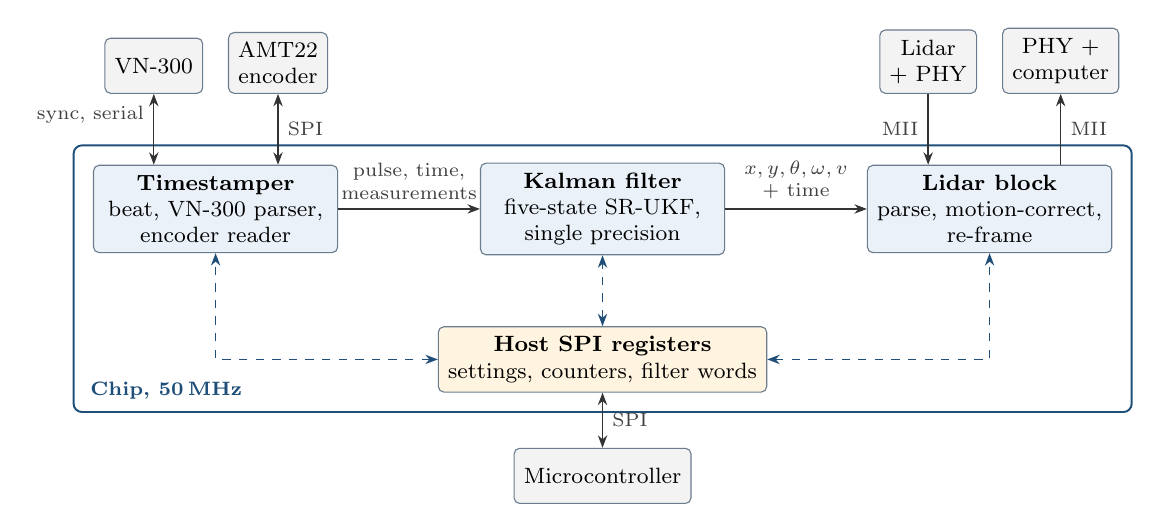
\begin{tikzpicture}[node distance=5mm and 14mm]
  % chip blocks
  \node[box,minimum width=31mm] (ts) {\textbf{Timestamper}\\beat, VN-300 parser,\\encoder reader};
  \node[box,minimum width=31mm,right=18mm of ts] (kf) {\textbf{Kalman filter}\\five-state SR-UKF,\\single precision};
  \node[box,minimum width=31mm,right=18mm of kf] (lb) {\textbf{Lidar block}\\parse, motion-correct,\\re-frame};
  \node[ctlb,minimum width=31mm,below=9mm of kf] (reg) {\textbf{Host SPI registers}\\settings, counters, filter words};
  \begin{scope}[on background layer]
    \node[draw=accent,line width=0.7pt,rounded corners=3pt,fit=(ts)(lb)(reg),inner sep=7pt,
          ] (chip) {};
    \node[font=\scriptsize\bfseries,text=accent,anchor=south west] at ($(chip.south west)+(1mm,0.5mm)$) {Chip, 50\,MHz};
  \end{scope}
  % externals
  \node[extb,above left=9mm and -14mm of ts] (vn) {VN-300};
  \node[extb,above right=9mm and -14mm of ts] (enc) {AMT22\\encoder};
  \node[extb,above left=9mm and -14mm of lb] (lid) {Lidar\\+ PHY};
  \node[extb,above right=9mm and -14mm of lb] (pc) {PHY +\\computer};
  \node[extb,below=7mm of reg] (mcu) {Microcontroller};
  % wires
  \draw[data,<->] (vn) -- node[lab,left,pos=0.3]{sync, serial} (vn|-ts.north);
  \draw[data,<->] (enc) -- node[lab,right]{SPI} (enc|-ts.north);
  \draw[data] (lid) -- node[lab,left]{MII} (lid|-lb.north);
  \draw[data] (pc|-lb.north) -- node[lab,right]{MII} (pc);
  \draw[data] (ts) -- node[lab,above]{pulse, time,\\measurements} (kf);
  \draw[data] (kf) -- node[lab,above]{$x,y,\theta,\omega,v$\\+ time} (lb);
  \draw[data,<->] (mcu) -- node[lab,right]{SPI} (reg);
  \draw[ctrl,<->] (reg) -- (kf);
  \draw[ctrl,<->] (reg.west) -| (ts.south);
  \draw[ctrl,<->] (reg.east) -| (lb.south);
\end{tikzpicture}
\caption{System. Solid: data. Dashed: settings in, status out. PHY: Ethernet physical-layer transceiver. MII: media-independent interface, the 4-bit link between a PHY and the chip. SPI: serial peripheral interface.}
\label{fig:system}
\end{figure}

\section{Architecture}

\subsection{Timestamper: one instant for every measurement}
A filter that fuses two sensors needs to know they describe the same moment. Left free-running,
the VN-300 and the encoder would be sampled up to one period (2.5\,ms) apart, and the lidar would
have no clock in common with either. The timestamper therefore owns time for the whole chip
(Fig.~\ref{fig:ts}). Every 2,500\,\textmu s it pulses the VN-300's sync input, which triggers that
sensor's measurement, and starts the encoder read in the same clock. It checks the VN-300
message's CRC (cyclic redundancy check) and the encoder's parity bits, and hands the filter one
pulse with a valid bit per sensor. A deadline of 2,000\,\textmu s bounds the wait: a late or
corrupted sensor costs that sensor's update for one beat and never stalls the filter. The same
microsecond counter stamps lidar sweeps.

\begin{figure}[!htb]
\centering
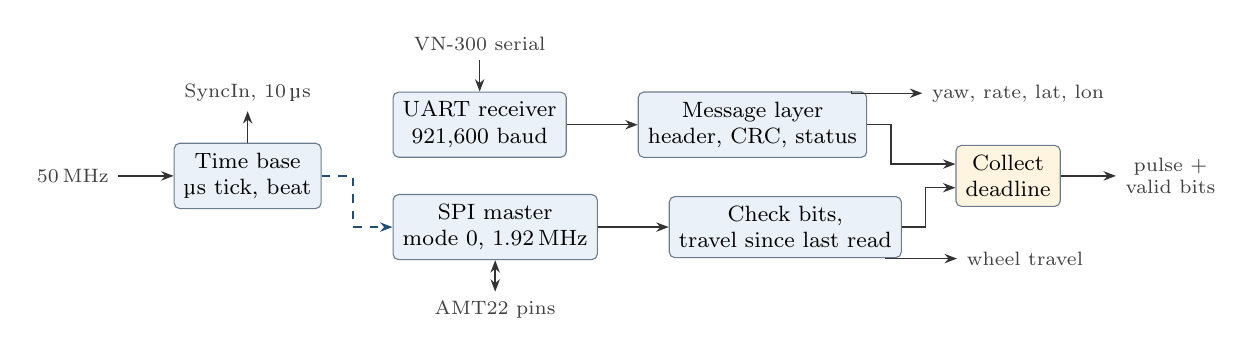
\begin{tikzpicture}[node distance=3.5mm and 9mm]
  \node[box] (tb) {Time base\\\textmu s tick, beat};
  \node[box,right=of tb,yshift=6.5mm] (uart) {UART receiver\\921,600 baud};
  \node[box,right=of tb,yshift=-6.5mm] (spi) {SPI master\\mode 0, 1.92\,MHz};
  \node[box,right=of uart] (msg) {Message layer\\header, CRC, status};
  \node[box,right=of spi] (dw) {Check bits,\\travel since last read};
  \node[ctlb,right=9mm of $(msg.east)!0.5!(dw.east)$] (col) {Collect\\deadline};
  \node[lab,left=7mm of tb] (osc) {50\,MHz};
  \node[lab,above=4mm of uart] (vn) {VN-300 serial};
  \node[lab,below=4mm of spi] (enc) {AMT22 pins};
  \node[lab,above=4mm of tb] (sync) {SyncIn, 10\,\textmu s};
  \node[lab,right=7mm of col] (out) {pulse +\\valid bits};
  \node[lab,right=7mm of msg,yshift=4mm] (m1) {yaw, rate, lat, lon};
  \node[lab,right=7mm of dw,yshift=-4mm] (m2) {wheel travel};
  \draw[data] (osc) -- (tb); \draw[data] (tb) -- (sync);
  \draw[data] (vn) -- (uart); \draw[data,<->] (enc) -- (spi);
  \draw[ctrl] (tb.east) -- ++(4mm,0) |- (spi.west);
  \draw[data] (uart) -- (msg); \draw[data] (spi) -- (dw);
  \draw[data] (msg.east) -- ++(3mm,0) |- ($(col.west)+(0,1.5mm)$);
  \draw[data] (dw.east) -- ++(3mm,0) |- ($(col.west)+(0,-1.5mm)$);
  \draw[data] (col) -- (out);
  \draw[data] (msg.north east) ++(-2mm,0) |- (m1.west);
  \draw[data] (dw.south east) ++(-2mm,0) |- (m2.west);
\end{tikzpicture}
\caption{Timestamper. The beat (dashed) starts the encoder read and the sync pulse together.}
\label{fig:ts}
\end{figure}

\subsection{Kalman filter}

\textbf{Conventions.} Position is $x$ east and $y$ north of the first position fix, in metres.
Heading $\theta$ is measured from east and is positive anticlockwise, so turning from east towards
north increases $\theta$; the turn rate $\omega$ has the same sign. The state is
$\mathbf{x}=[x,\;y,\;\theta,\;\omega,\;r]^{\mathsf T}$, where $r$ is the dead wheel's radius.

\textbf{Prediction} carries the estimate from beat $k-1$ to beat $k$ using the wheel rotation
$\Delta\phi_k$ measured in that beat and $\Delta t=2.5$\,ms. A superscript minus marks a value
predicted before the measurements of beat $k$ are applied:
\begin{align*}
\bar\theta &= \theta_{k-1}+\tfrac12\,\omega_{k-1}\Delta t &&\text{heading at the middle of the beat}\\
x_k^- &= x_{k-1}+r_{k-1}\,\Delta\phi_k\cos\bar\theta, \qquad
y_k^- = y_{k-1}+r_{k-1}\,\Delta\phi_k\sin\bar\theta &&\text{distance rolled, along that heading}\\
\theta_k^- &= \theta_{k-1}+\omega_{k-1}\Delta t, \qquad \omega_k^-=\omega_{k-1}, \qquad r_k^-=r_{k-1}
\end{align*}
\textbf{Correction} applies the VN-300's four readings $z_i$ (position east, position north,
heading, turn rate), each of which measures one state directly, with noise variance $R_i$. With
$P=S^{\mathsf T}S$ the covariance, for $i=1\ldots4$ in turn:
\begin{equation*}
e = z_i - x_i^- \;\;(\text{wrapped to } (-\pi,\pi] \text{ for heading}), \qquad
\mathbf{k} = \frac{P_{\cdot i}}{P_{ii}+R_i}, \qquad
\mathbf{x}\leftarrow\mathbf{x}+\mathbf{k}\,e, \qquad
P\leftarrow P-\mathbf{k}\,P_{i\cdot} .
\end{equation*}
The VN-300 reports yaw in degrees clockwise from north, so the filter converts it with
$\theta=\pi/2-\text{yaw}$ (in radians) and flips the sign of the turn rate.

\textbf{Why this filter, built this way.} Each choice below was made against a concrete
alternative.

\begin{center}\footnotesize
\begin{tabularx}{\linewidth}{@{}p{0.2\linewidth}p{0.2\linewidth}X@{}}
\toprule
Choice & Alternative & Reason\\
\midrule
Wheel radius as the fifth state & Fixed radius, or an additive speed bias &
Odometry error from a worn or mis-measured wheel is a scale error. Estimating the scale lets
satellite positioning calibrate the wheel, so dead reckoning stays accurate when the fix is lost.\\
Unscented filter & Extended Kalman filter &
No Jacobians: the motion model is one subroutine, called once per sigma point. On this machine
extra evaluations cost time, which is spare, not area.\\
Square-root form & Propagating $P$ &
In single precision $P$ can lose symmetry or go indefinite. Carrying $S$ keeps $P=S^{\mathsf T}S$
valid by construction and halves the dynamic range of the numbers.\\
Single precision floating point & 32-bit fixed point &
Simulation showed fixed point loses the small corrections made at 400\,Hz; single precision
matches double.\\
Four scalar corrections & One $4\times4$ update &
Each measurement reads one state and their noises are independent, so the results are identical,
and no matrix solve or QR factorisation is needed.\\
Rank-one updates of $S$ & QR factorisation of all sigma points &
Same factor, one small routine reused 11 times, and the 11 sigma points need never be stored:
they are regenerated, which saves 55 words of storage for about twice the model evaluations.\\
Sine and cosine by series & CORDIC block &
A six-term Maclaurin series after folding into $\pm\pi/2$ runs on the existing arithmetic unit
and reaches single-precision resolution (error $6\times10^{-8}$). It adds about 20 steps and no hardware.\\
\bottomrule
\end{tabularx}
\end{center}

\textbf{A stored-program machine, not a datapath.} The team's first design used a dedicated
multiply-accumulate unit and a divide/square-root unit. The filter needs about 3,200 operations
per beat and has 125,000 clocks to do them in, so any unit faster than about 39 clocks per
operation buys nothing. The chip instead has one bit-serial unit built around a single 29-bit
adder (30 to 80 clocks per operation), a table of 545 steps of the form $d=a\;\mathrm{op}\;b$, and
63 words of latch storage (Fig.~\ref{fig:machine}). An update takes 93,000 clocks, 1.86\,ms of the
2.5\,ms beat. Two further benefits follow from the program being data: it is generated by a
Python script that is also a bit-exact model of the machine, so the tested program is the one on
the chip; and eight of its constants (noise settings, encoder scale, starting radius) are
host-writable, so the filter can be retuned on the bench without new silicon.

\begin{figure}[!htb]
\centering
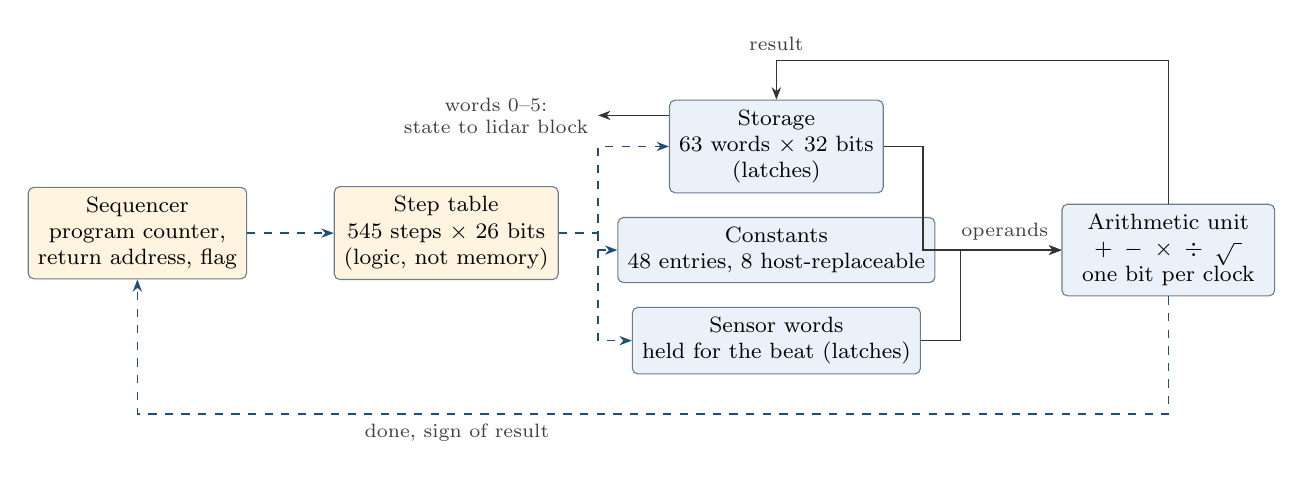
\begin{tikzpicture}[node distance=6mm and 11mm]
  \node[ctlb,minimum width=24mm] (pc) {Sequencer\\program counter,\\return address, flag};
  \node[ctlb,minimum width=24mm,right=of pc] (rom) {Step table\\545 steps $\times$ 26 bits\\(logic, not memory)};
  \node[box,minimum width=26mm,right=14mm of rom,yshift=11mm] (store) {Storage\\63 words $\times$ 32 bits\\(latches)};
  \node[box,minimum width=26mm,below=3mm of store] (const) {Constants\\48 entries, 8 host-replaceable};
  \node[box,minimum width=26mm,below=3mm of const] (sens) {Sensor words\\held for the beat (latches)};
  \node[box,minimum width=27mm,right=16mm of const] (fp) {Arithmetic unit\\$+\;-\;\times\;\div\;\sqrt{\ }$\\one bit per clock};
  \draw[ctrl] (pc) -- (rom);
  \draw[ctrl] (rom.east) -- ++(5mm,0) coordinate (f) |- (store.west);
  \draw[ctrl] (f) |- (const.west);
  \draw[ctrl] (f) |- (sens.west);
  \draw[data] (store.east) -- ++(5mm,0) coordinate (m) |- (fp.west);
  \draw[data] (const.east) -- (fp.west);
  \draw[data] (sens.east) -- ++(5mm,0) |- (fp.west);
  \node[lab,above=0pt of $(const.east)!0.55!(fp.west)$] {operands};
  \draw[data] (fp.north) |- ($(store.north)+(0,5mm)$) -| node[lab,pos=0.25,above]{result} (store.north);
  \draw[ctrl] (fp.south) |- ($(sens.south)+(0,-5mm)$) -| node[lab,pos=0.25,below]{done, sign of result} (pc.south);
  \draw[data] (store.north west) ++(0,-2mm) -- ++(-9mm,0) node[lab,left]{words 0--5:\\state to lidar block};
\end{tikzpicture}
\caption{The filter machine. Dashed: control and addresses. Solid: 32-bit data.}
\label{fig:machine}
\end{figure}

\subsection{Lidar block}

\textbf{What the lidar sends.} A Velodyne VLP-16 spins 16 lasers at 10 revolutions per second. It
streams about 754 UDP packets per second, each a 1,206-byte payload of 12 blocks. A block is one
azimuth reading followed by 32 returns (two firings of the 16 lasers), each a distance in 2\,mm
units and a reflectivity:

\begin{center}
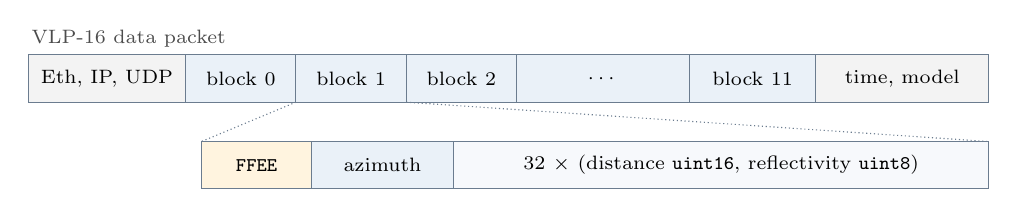
\begin{tikzpicture}[x=1mm,y=1mm,font=\scriptsize]
  \node[anchor=south west,text=black!70,inner sep=1pt] at (0,6.5) {VLP-16 data packet};
  \draw[fill=ext,draw=rule] (0,0) rectangle (20,6) node[midway]{Eth, IP, UDP};
  \foreach \i in {0,1,2} \draw[fill=blk,draw=rule] (20+\i*14,0) rectangle (34+\i*14,6) node[midway]{block \i};
  \draw[fill=blk,draw=rule] (62,0) rectangle (84,6) node[midway]{$\cdots$};
  \draw[fill=blk,draw=rule] (84,0) rectangle (100,6) node[midway]{block 11};
  \draw[fill=ext,draw=rule] (100,0) rectangle (122,6) node[midway]{time, model};
  \draw[rule,densely dotted] (34,0) -- (22,-5); \draw[rule,densely dotted] (48,0) -- (122,-5);
  \draw[fill=ctl,draw=rule] (22,-11) rectangle (36,-5) node[midway]{\texttt{FFEE}};
  \draw[fill=blk,draw=rule] (36,-11) rectangle (54,-5) node[midway]{azimuth};
  \draw[fill=blk!40,draw=rule] (54,-11) rectangle (122,-5) node[midway]{32 $\times$ (distance \texttt{uint16}, reflectivity \texttt{uint8})};
\end{tikzpicture}
\end{center}

That is 290,000 returns per second in polar form, and one sweep of about 29,000 returns takes
100\,ms to collect.

\textbf{The problem.} Returns are measured relative to wherever the robot is at the instant each
laser fires, but a sweep is used as if it were taken from one pose (Fig.~\ref{fig:smear}). A
return at range $R$ taken a time $t$ after the sweep started is misplaced by about
$R\,\omega\,t$ sideways and $v\,t$ along the direction of travel. For a robot turning at
$90^\circ$/s (1.57\,rad/s) and driving at 2\,m/s, by the end of a sweep ($t=0.1$\,s) it has turned
$9^\circ$:
\begin{equation*}
R\,\omega\,t = 10\,\text{m}\times1.57\,\text{rad/s}\times0.1\,\text{s}\approx 1.6\,\text{m},
\qquad v\,t = 2\,\text{m/s}\times0.1\,\text{s}=0.2\,\text{m}.
\end{equation*}
The lidar's distance unit is 2\,mm. To keep the error at 10\,m under even 1\,cm the robot would
have to turn slower than $0.6^\circ$/s, so for a robot that manoeuvres the correction is not
optional: without it walls bend and obstacles appear up to metres from where they are.

\begin{figure}[!htb]
\centering
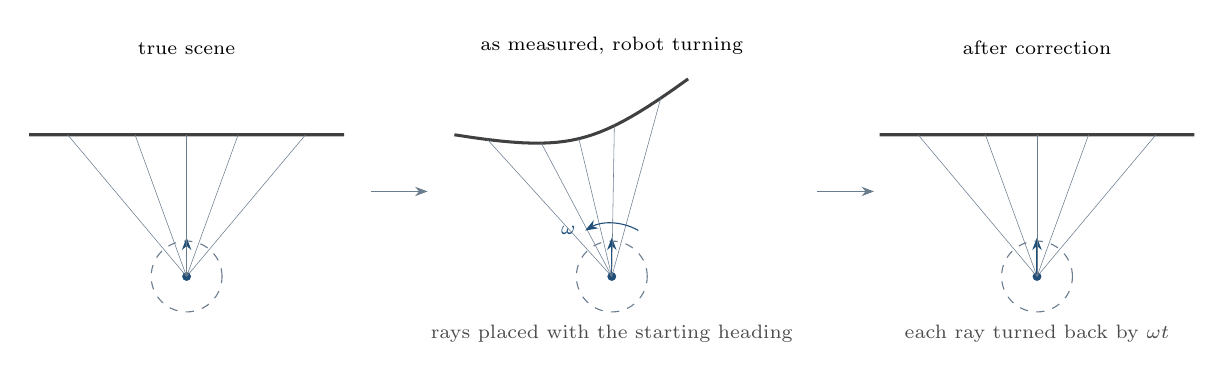
\begin{tikzpicture}[x=9mm,y=9mm,font=\scriptsize]
  \foreach \ox/\ttl/\k in {0/{true scene}/0, 6/{as measured, robot turning}/0.28, 12/{after correction}/0} {
    \begin{scope}[shift={(\ox,0)}]
      \node[anchor=south] at (0,3.0) {\ttl};
      \draw[rule,dashed] (0,0) circle (0.5);
      \fill[accent] (0,0) circle (1.6pt); \draw[accent,->] (0,0) -- (0,0.55);
      \draw[line width=1.1pt,black!75] plot[domain=-48:48,samples=25] ({2/cos(\x)*sin(\x-\k*(\x+48))},{2/cos(\x)*cos(\x-\k*(\x+48))});
      \foreach \a in {-40,-20,0,20,40} \draw[rule,very thin] (0,0) -- ({2/cos(\a)*sin(\a-\k*(\a+48))},{2/cos(\a)*cos(\a-\k*(\a+48))});
    \end{scope}}
  \draw[->,accent] (6,0) ++(60:0.75) arc (60:120:0.75) node[left,text=accent]{$\omega$};
  \draw[->,rule] (2.6,1.2) -- (3.4,1.2); \draw[->,rule] (8.9,1.2) -- (9.7,1.2);
  \node[below,text=black!70] at (6,-0.55) {rays placed with the starting heading};
  \node[below,text=black!70] at (12,-0.55) {each ray turned back by $\omega t$};
\end{tikzpicture}
\caption{Why a sweep needs the filter state. A straight wall, scanned left to right while the
robot turns, comes out rotated and stretched because later rays are measured from a later heading (turn exaggerated).}
\label{fig:smear}
\end{figure}

\textbf{The method.} For every firing the block keeps running totals of how far the robot has
turned ($\omega$ per firing period) and moved ($v$ per firing period) since the sweep started. A
CORDIC (shift-and-add rotation) unit gives the sine and cosine of the lidar azimuth minus the
angle turned, each return is converted to $x,y,z$ and the movement is added
(Fig.~\ref{fig:lidar}). Every sweep is thus expressed in the robot's frame at the moment the sweep
started. This path is 16-bit fixed point with its own multiplier, because 172 clocks per return
is far too few for the filter's serial unit.

\begin{figure}[!htb]
\centering
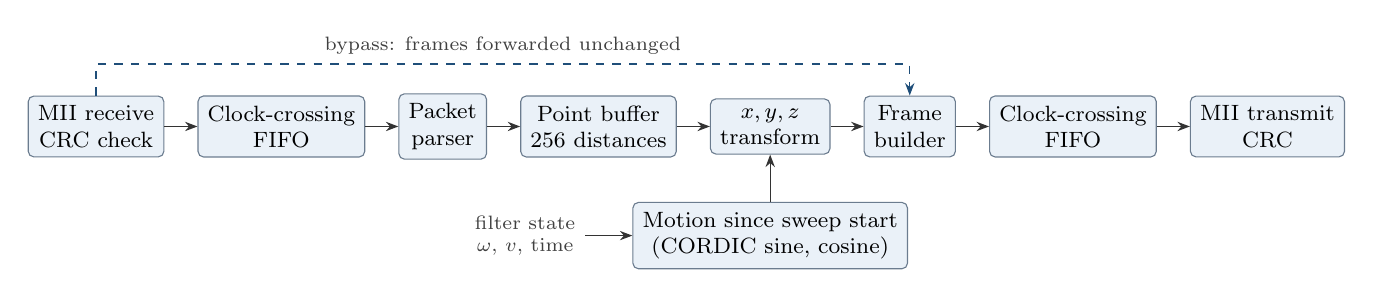
\begin{tikzpicture}[node distance=4mm and 4.2mm]
  \node[box] (rx) {MII receive\\CRC check};
  \node[box,right=of rx] (f1) {Clock-crossing\\FIFO};
  \node[box,right=of f1] (pp) {Packet\\parser};
  \node[box,right=of pp] (pb) {Point buffer\\256 distances};
  \node[box,right=of pb] (xyz) {$x,y,z$\\transform};
  \node[box,right=of xyz] (fb) {Frame\\builder};
  \node[box,right=of fb] (f2) {Clock-crossing\\FIFO};
  \node[box,right=of f2] (tx) {MII transmit\\CRC};
  \node[box,below=6mm of xyz] (mo) {Motion since sweep start\\(CORDIC sine, cosine)};
  \node[lab,left=6mm of mo] (st) {filter state\\$\omega$, $v$, time};
  \foreach \a/\b in {rx/f1,f1/pp,pp/pb,pb/xyz,xyz/fb,fb/f2,f2/tx} \draw[data] (\a) -- (\b);
  \draw[data] (mo) -- (xyz);
  \draw[data] (st) -- (mo);
  \draw[ctrl] (rx.north) -- ++(0,4mm) -| node[lab,pos=0.25,above]{bypass: frames forwarded unchanged} (fb.north);
\end{tikzpicture}
\caption{Lidar path. The two MII sides run on their own 25\,MHz clocks.}
\label{fig:lidar}
\end{figure}

\textbf{Why the filter and the lidar path share a chip.} The correction needs $\omega$ and $v$ at
the time of each firing, on the same clock as the lidar data. On the chip the state is at most
2.5\,ms old (40 updates per sweep) and is timed by the same microsecond counter that stamps the
sweep, with no network or operating-system delay in between. The alternative is to forward raw
packets and correct on the computer, which needs the two data streams aligned after Ethernet and
scheduler jitter, and repeats the trigonometry on the CPU for every return. The cost of the
tight coupling is that a wrong state bends the point cloud. Three things limit that risk: the
turning and moving corrections are switched on separately, the host can supply the state
instead of the filter, and the lidar block can be bypassed so that frames pass through
untouched. The state used is also carried in every packet header, so the computer can place each
sweep in the world and can check the correction.

\section{Physical design}

The design was built with the Tiny Tapeout LibreLane flow. Fitting it in $8\times4$ tiles was the
main difficulty: the chip is limited by routing congestion, not by timing.

\begin{center}\small
\begin{tabular}{@{}lr@{\qquad\qquad}lr@{}}
\toprule
Die & $1.378\times0.511$\,mm & Clock & 50\,MHz (20\,ns)\\
Core area & 0.694\,mm$^2$ & Setup slack, typical (1.80\,V, 25\,\textdegree C) & $+8.94$\,ns\\
Placement utilisation & 78.2\,\% & Setup slack, slow (1.60\,V, 100\,\textdegree C) & $+3.33$\,ns\\
Logic cells & 58,100 & Worst hold slack, nine corners & $+0.10$\,ns\\
Flip-flops / latches & 3,747 / 6,484 & Routed wire & 2.1\,m\\
\bottomrule
\end{tabular}
\end{center}

\begin{figure}[!htb]
\centering
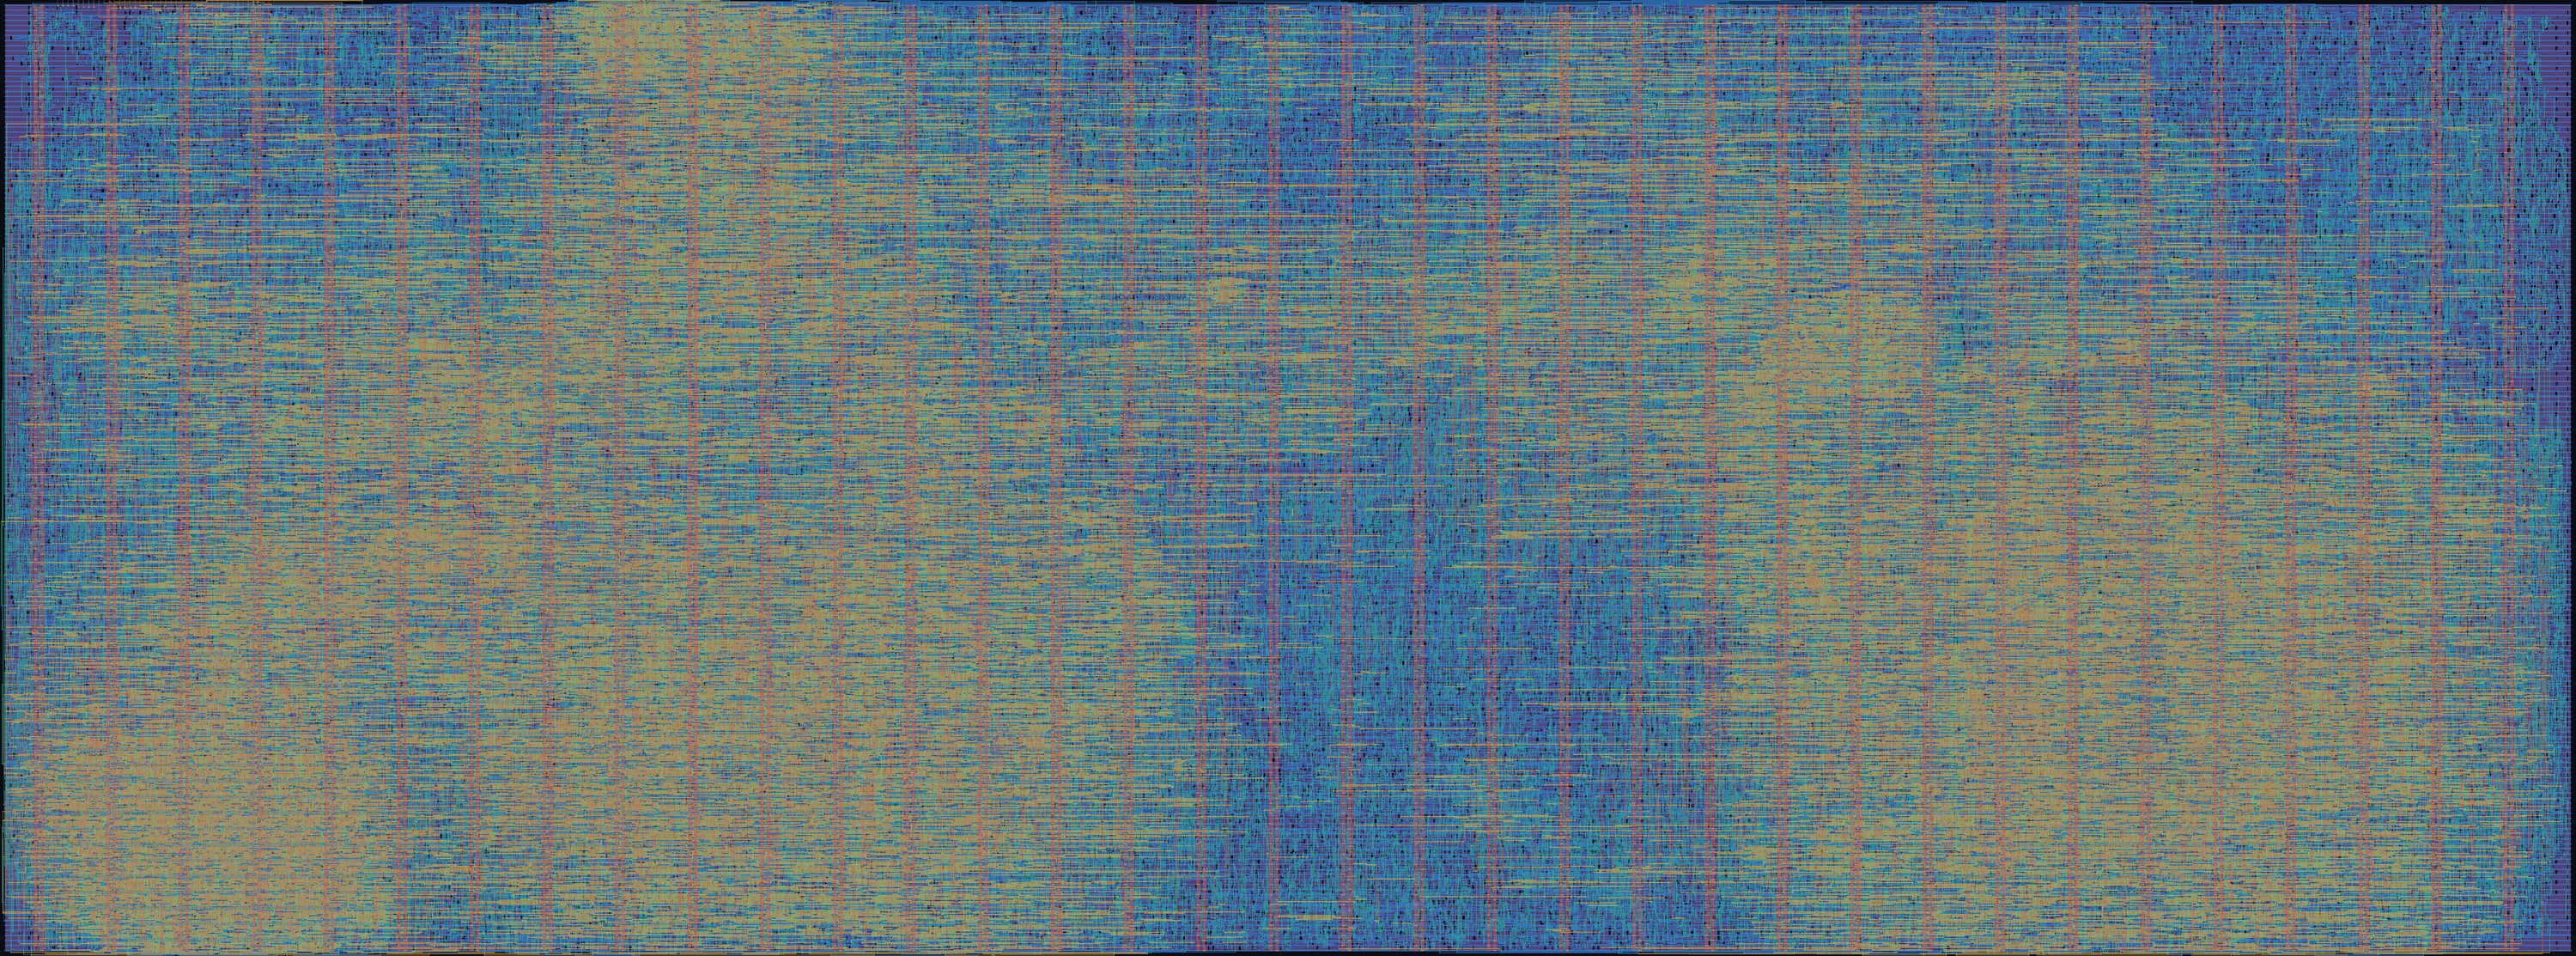
\includegraphics[width=0.495\linewidth]{dieshot.jpg}\hfill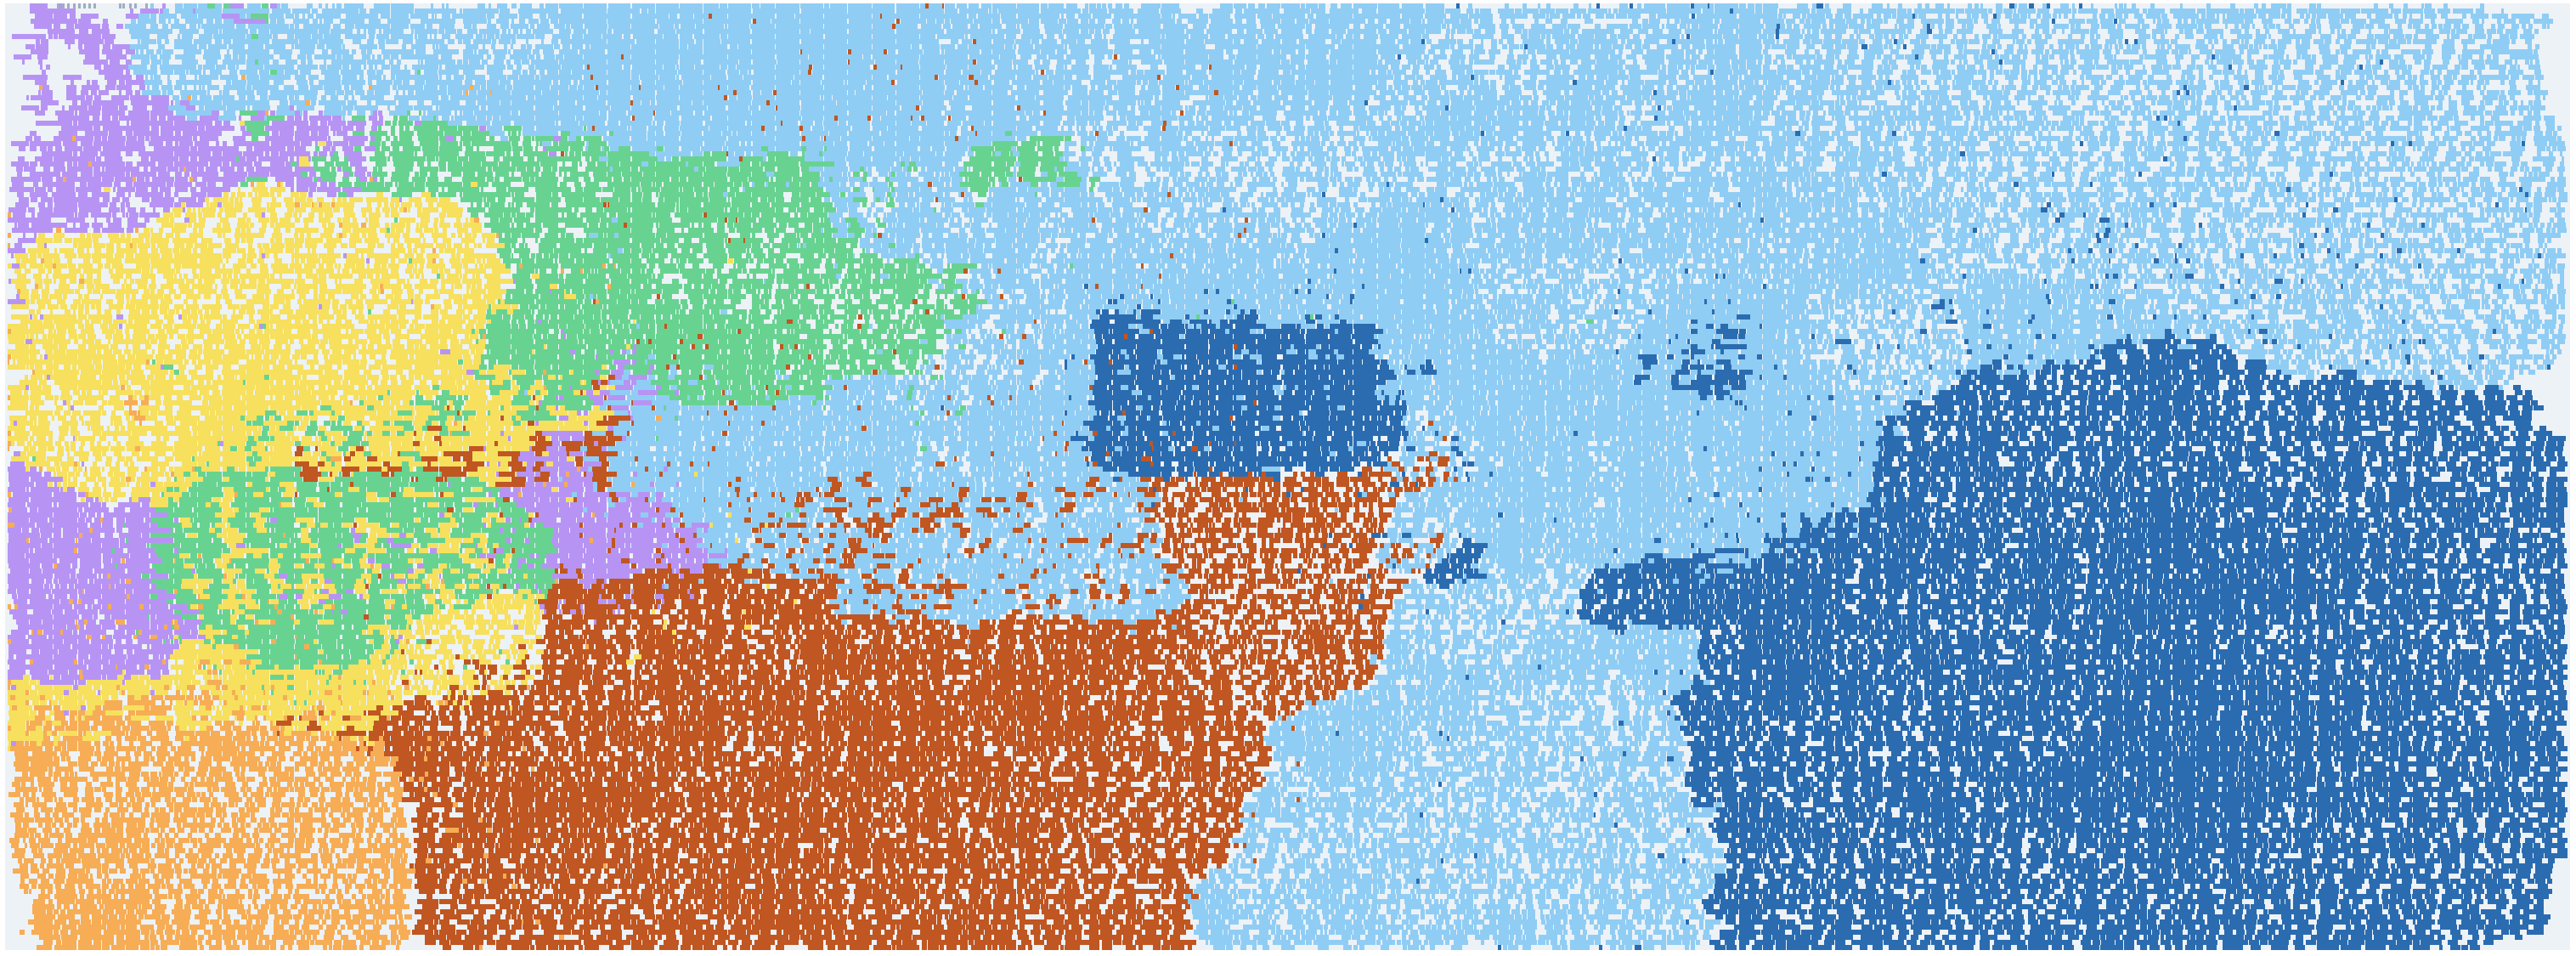
\includegraphics[width=0.495\linewidth]{floorplan.png}\\[3pt]
{\scriptsize
\newcommand{\sw}[2]{\tikz[baseline=-0.6ex]\fill[#1] (0,-0.9mm) rectangle (2.6mm,0.9mm);\,#2\quad}
\definecolor{fpA}{HTML}{90CDF4}\definecolor{fpB}{HTML}{2B6CB0}\definecolor{fpC}{HTML}{C05621}\definecolor{fpD}{HTML}{F6AD55}
\definecolor{fpE}{HTML}{F6E05E}\definecolor{fpF}{HTML}{68D391}\definecolor{fpG}{HTML}{B794F4}
\sw{fpA}{lidar logic 41\,\%}\sw{fpB}{lidar point buffer 23\,\%}\sw{fpC}{filter storage 14\,\%}\sw{fpD}{step table 4\,\%}\\[1pt]
\sw{fpE}{filter arithmetic and sequencer 7\,\%}\sw{fpF}{host registers 7\,\%}\sw{fpG}{timestamper 4\,\%}}
\caption{The final layout. Left: metal layers, local interconnect (violet) up to the metal-4 power
straps (red). Right: the same area with each cell coloured by block; shares are of logic cell
area. Cells without a block name are assigned by connectivity, so boundaries are approximate.}
\label{fig:layout}
\end{figure}

\subsection{Latch storage}
The filter's 71 words, the lidar's 256-word point buffer and the held sensor words are
\texttt{dlxtp\_1} latches placed by name: 6,484 bits, each a quarter to 40\,\% smaller than a
flip-flop. No clock is gated. One flip-flop on the falling edge makes a one-clock pulse for the
whole memory, and an AND gate per word combines it with that word's select
(Fig.~\ref{fig:latch}). The select and the data come from registers that hold until the next
write, so they are steady for half a clock before the enable rises and well after it falls. Both
margins hold by construction and do not depend on the tools checking latch timing.

\begin{figure}[!htb]
\centering
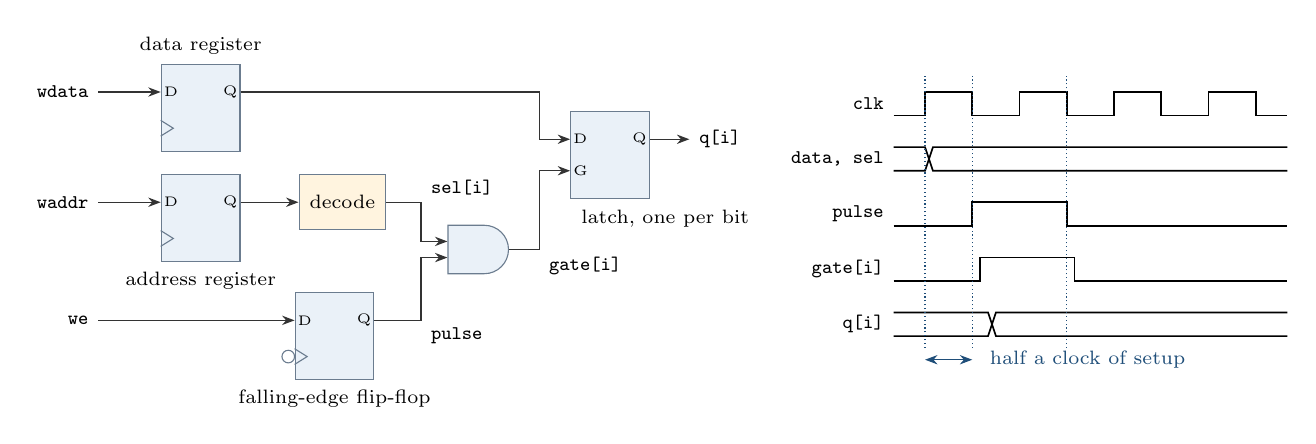
\begin{tikzpicture}[circuit logic US,x=1mm,y=1mm,font=\scriptsize]
  \newcommand{\cell}[4]{% name, centre, lower-left label, bubble (0/1)
    \node[ff,minimum width=10mm,minimum height=11mm] (#1) at (#2) {};
    \node[font=\tiny,anchor=west,inner sep=1pt] at ($(#1.west)+(0,2)$) {D};
    \node[font=\tiny,anchor=east,inner sep=1pt] at ($(#1.east)+(0,2)$) {Q};
    #3}
  \newcommand{\ck}[1]{\draw[rule] ($(#1.west)+(0,-1.6)$) -- ++(1.6,-1) -- ++(-1.6,-1);}
  \cell{r1}{0,14}{\ck{r1}}{}
  \cell{r2}{0,0}{\ck{r2}}{}
  \cell{p}{17,-15}{\ck{p}\draw[rule,fill=white] ($(p.west)+(-0.8,-2.6)$) circle (0.8);}{}
  \cell{l}{52,8}{\node[font=\tiny,anchor=west,inner sep=1pt] at ($(l.west)+(0,-2)$) {G};}{}
  \node[draw=rule,fill=ctl,minimum width=11mm,minimum height=7mm] (dec) at (18,2) {decode};
  \node[and gate,draw=rule,fill=blk,inputs=nn] (g) at (35,-4) {};
  \node[above=0pt of r1] {data register};
  \node[below=0pt of r2] {address register};
  \node[below=0pt of p] {falling-edge flip-flop};
  \node[anchor=north west,inner sep=1pt] at ($(l.south west)+(1,-1)$) {latch, one per bit};
  \draw[data] (-13,16) node[left]{\texttt{wdata}} -- ($(r1.west)+(0,2)$);
  \draw[data] (-13,2) node[left]{\texttt{waddr}} -- ($(r2.west)+(0,2)$);
  \draw[data] (-13,-13) node[left]{\texttt{we}} -- ($(p.west)+(0,2)$);
  \draw[data] ($(r1.east)+(0,2)$) -- (43,16) |- ($(l.west)+(0,2)$);
  \draw[data] ($(r2.east)+(0,2)$) -- (dec.west);
  \draw[data] (dec.east) -- (28,2) node[above right=-1pt and 0pt]{\texttt{sel[i]}} |- (g.input 1);
  \draw[data] ($(p.east)+(0,2)$) -- (28,-13) node[below right=-1pt and 0pt]{\texttt{pulse}} |- (g.input 2);
  \draw[data] (g.output) -- (43,-4) node[below right=-1pt and 0pt]{\texttt{gate[i]}} |- ($(l.west)+(0,-2)$);
  \draw[data] ($(l.east)+(0,2)$) -- ++(5,0) node[right]{\texttt{q[i]}};
  % waveforms
  \begin{scope}[shift={(88,-15)}]
    \foreach \y/\n in {28/clk,21/data{,} sel,14/pulse,7/gate[i],0/q[i]} \node[left] at (0,\y+1.5) {\texttt{\n}};
    \draw[wv] (0,28)--(4,28)--(4,31)--(10,31)--(10,28)--(16,28)--(16,31)--(22,31)--(22,28)--(28,28)--(28,31)--(34,31)--(34,28)--(40,28)--(40,31)--(46,31)--(46,28)--(50,28);
    \draw[wv] (0,21)--(4,21)--(5,24)--(50,24); \draw[wv] (0,24)--(4,24)--(5,21)--(50,21);
    \draw[wv] (0,14)--(10,14)--(10,17)--(22,17)--(22,14)--(50,14);
    \draw[wv] (0,7)--(11,7)--(11,10)--(23,10)--(23,7)--(50,7);
    \draw[wv] (0,0)--(12,0)--(13,3)--(50,3); \draw[wv] (0,3)--(12,3)--(13,0)--(50,0);
    \draw[accent,densely dotted] (4,-1.5)--(4,33); \draw[accent,densely dotted] (10,-1.5)--(10,33); \draw[accent,densely dotted] (22,-1.5)--(22,33);
    \draw[accent,<->] (4,-3)--(10,-3); \node[text=accent,anchor=west] at (11,-3) {half a clock of setup};
  \end{scope}
\end{tikzpicture}
\caption{Writing a latch word without a gated clock, and its timing.}
\label{fig:latch}
\end{figure}

An earlier version used a clock gate per word. The tools treated the 256 gated clocks as clock
nets, gave each wide wiring, and could not route the result. The same latches hold the VN-300
words for the duration of a filter update; doing that in 116 flip-flops instead put utilisation
at 78.65\,\% and detailed routing never converged, where latches give 78.23\,\% and route cleanly.

\subsection{Read paths and two-clock paths}
Reading a latch memory is a wide selector. Left alone, the tools build it flat, and wherever its
words land far apart a small gate is left driving millimetres of wire. The selector is therefore
built in two levels with \texttt{buf\_4} cells instantiated by name between them
(Fig.~\ref{fig:read}), which also gives the timing constraints fixed pins to refer to.

\begin{figure}[!htb]
\centering
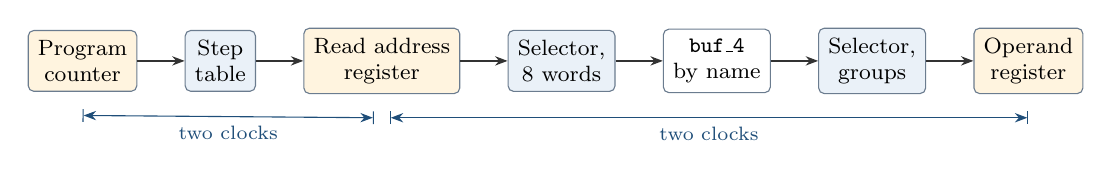
\begin{tikzpicture}[node distance=4mm and 6mm]
  \node[ctlb] (pc) {Program\\counter};
  \node[box,right=of pc] (rom) {Step\\table};
  \node[ctlb,right=of rom] (ra) {Read address\\register};
  \node[box,right=of ra] (m1) {Selector,\\8 words};
  \node[box,right=of m1,fill=white] (b) {\texttt{buf\_4}\\by name};
  \node[box,right=of b] (m2) {Selector,\\groups};
  \node[ctlb,right=of m2] (fp) {Operand\\register};
  \foreach \a/\b in {pc/rom,rom/ra,ra/m1,m1/b,b/m2,m2/fp} \draw[data] (\a) -- (\b);
  \draw[accent,|<->|] ($(pc.south)+(0,-3mm)$) -- node[lab,below,text=accent]{two clocks} ($(ra.south)+(-1mm,-3mm)$);
  \draw[accent,|<->|] ($(ra.south)+(1mm,-3mm)$) -- node[lab,below,text=accent]{two clocks} ($(fp.south)+(0,-3mm)$);
\end{tikzpicture}
\caption{The filter's read path. Yellow: registers. The sequencer waits a clock after the counter changes, and takes a word only after its address has been steady for a full clock.}
\label{fig:read}
\end{figure}

Four paths are too long for one 20\,ns clock at the slow corner: the two in
Fig.~\ref{fig:read}, the lidar buffer read and the SPI read address. On each the logic waits one
extra clock, and the constraints declare a two-clock path (\texttt{set\_multicycle\_path}) through
named nets and the named buffer pins. In simulation the value is forced unknown during the wait,
so any logic that used it early would fail the tests.

\section{Future-proofing}

The filter's program is fixed in the layout, so flexibility was put where it costs little.
\begin{itemize}
\item \textbf{Tuning without a respin.} Noise settings, encoder scale and starting wheel radius are
host-writable, and beat period and deadline are registers.
\item \textbf{Full observability.} Every storage word, constant and sensor word of the filter can be
read over SPI, so a wrong result on the bench can be traced to a step.
\item \textbf{Fallbacks.} The host can supply the state itself (control bit 7), so the lidar
correction still works if the filter or a sensor assumption turns out wrong. The lidar block can
be bypassed entirely, and the timestamper works alone.
\item \textbf{Other sensors.} A different odometry source, such as stereo visual odometry, can be
fed in by a microcontroller that answers as the AMT22 encoder, or fused in a host-side filter that
writes the state.
\end{itemize}

\textbf{Limits of this chip.} Storage uses 63 of 64 words and an update takes 74\,\% of the beat. A
sixth state would need an update of roughly 3.2\,ms (estimate), which does not fit 400\,Hz, and a
host-writable step table would need about 45--50\,kbit of latches (estimate), which does not fit
the area.

\appendix
\section{Interface reference}

\subsection{Output packets}
The corrected points leave as ordinary UDP datagrams over 100\,Mbit Ethernet; a normal socket
receives them. Every datagram carries 1,224 bytes, little-endian (Fig.~\ref{fig:pkt}). The UDP
checksum is 0 (unused). Addresses and ports are registers (Table~\ref{tab:regs}).

\begin{figure}[!htb]
\centering
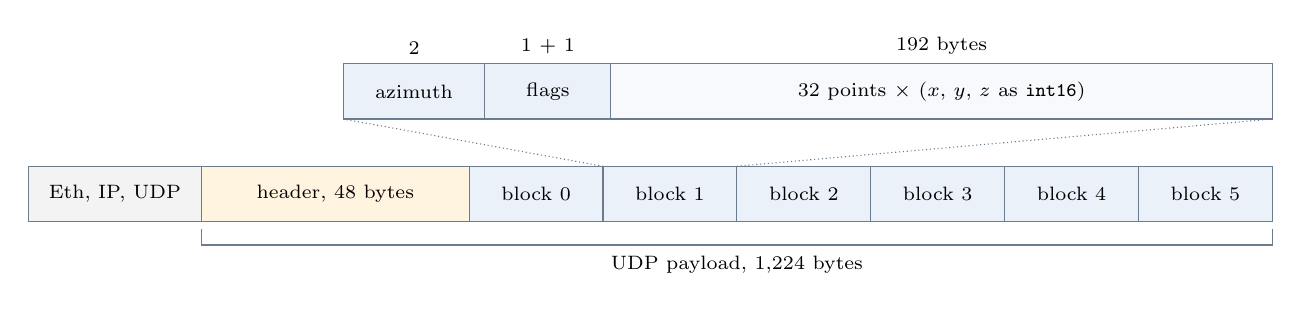
\begin{tikzpicture}[x=1mm,y=1mm,font=\scriptsize]
  \draw[fill=ext,draw=rule] (0,0) rectangle (22,7) node[midway]{Eth, IP, UDP};
  \draw[fill=ctl,draw=rule] (22,0) rectangle (56,7) node[midway]{header, 48 bytes};
  \foreach \i in {0,...,5} \draw[fill=blk,draw=rule] (56+\i*17,0) rectangle (73+\i*17,7) node[midway]{block \i};
  \draw[rule] (22,-1) -- (22,-3) -- (158,-3) -- (158,-1); \node at (90,-5.5) {UDP payload, 1,224 bytes};
  \draw[rule,densely dotted] (73,7) -- (40,13); \draw[rule,densely dotted] (90,7) -- (158,13);
  \draw[fill=blk,draw=rule] (40,13) rectangle (58,20) node[midway,align=center]{azimuth};
  \draw[fill=blk,draw=rule] (58,13) rectangle (74,20) node[midway]{flags};
  \draw[fill=blk!40,draw=rule] (74,13) rectangle (158,20) node[midway]{32 points $\times$ ($x$, $y$, $z$ as \texttt{int16})};
  \node[above] at (49,20) {2}; \node[above] at (66,20) {1 + 1}; \node[above] at (116,20) {192 bytes};
\end{tikzpicture}
\caption{One output datagram. A block is one azimuth reading of the lidar: 196 bytes.}
\label{fig:pkt}
\end{figure}

\begin{center}\footnotesize
\begin{tabular}{@{}rll@{\qquad}rll@{}}
\toprule
Offset & Field & Meaning & Offset & Field & Meaning\\
\midrule
0 & \texttt{magic} & ASCII \texttt{PC2X} & 17 & \texttt{point\_step} & bytes per point, 6\\
4 & \texttt{version} & 3 & 18 & \texttt{num\_blocks} & 6\\
5 & \texttt{flags} & see below & 19 & \texttt{points\_per\_block} & 32\\
6 & \texttt{num\_points} & 192 & 20 & \texttt{sweep\_time\_us} & chip time the sweep started\\
8 & \texttt{seq} & datagram counter & 24 & \texttt{state\_time\_us} & time of the state\\
12 & \texttt{sweep\_id} & sweep of the first block & 28--40 & \texttt{x}, \texttt{y}, \texttt{theta}, \texttt{omega} & \texttt{float32}: m, m, rad, rad/s\\
14 & \texttt{first\_azimuth} & 0.01\textdegree & 44 & \texttt{v} & \texttt{float32}, m/s\\
16 & \texttt{model} & lidar model & & &\\
\bottomrule
\end{tabular}
\end{center}

\begin{itemize}
\item \textbf{Header flags:} bit 0 a state has been received (if 0, points are uncorrected and
the state fields mean nothing); bit 1 one count is 4\,mm (else 2\,mm); bit 2 a lidar packet
arrived corrupted; bit 3 lidar data was discarded.
\item \textbf{Block flags:} bit 0 first block of a new sweep; bit 1 padding, skip the block.
\item \textbf{Points:} $x$ forward, $y$ left, $z$ up, in counts. $x=y=z=-32768$ means no return.
\end{itemize}

\subsection{Host interface}
The microcontroller is the SPI master: mode 0, most significant bit first, up to 5\,MHz. Byte 0 is
$\{\textit{write},\ \textit{address}[6{:}0]\}$; data bytes follow and the address counts up, so
several registers move in one transfer. Multi-byte numbers have the low byte at the lowest
address. Reset values let the chip run with no host attached. Table~\ref{tab:regs} is the register map.


\textbf{Control bits (register \texttt{02}).} 0 timestamper on; 1 lidar on; 2 lidar bypass; 3
output step 4\,mm; 4 correct for turning; 5 correct for moving; 6 check the encoder's turn bits;
7 lidar state comes from the filter (0: from \texttt{24}--\texttt{3B}). At reset bits 0, 1 and 6
are set, so the host must set bit 7 to use the filter and bits 4 and 5 to switch on correction.

\textbf{Counters (\texttt{40}--\texttt{46}).} Lidar packets, other frames, bad received checksums,
frames sent, buffer overflows, motion overruns, transmit underruns.

\begin{table}[H]
\centering\footnotesize
\caption{Register map. Addresses in hexadecimal; reset values in brackets.}
\label{tab:regs}
\begin{tabularx}{\linewidth}{@{}lX@{\quad}lX@{}}
\toprule
\texttt{00}, \texttt{01} & ID (\texttt{A7}) and version (\texttt{01}) &
\texttt{24}--\texttt{3B} & host-supplied state: time, $x$, $y$, $\theta$, $\omega$, $v$\\
\texttt{02} & control [\texttt{43}], bits below &
\texttt{3C}, \texttt{3D} & write: use the host state; clear the counters\\
\texttt{03} & lidar model [0]: VLP-16, Hi-Res, VLP-32C, HDL-32E &
\texttt{40}--\texttt{46} & event counters, read only, stop at 255\\
\texttt{04}--\texttt{05} & beat period, \textmu s [2500] &
\texttt{48}--\texttt{4B} & time of the last beat, \textmu s\\
\texttt{06}--\texttt{07} & measurement deadline, \textmu s [2000] &
\texttt{4C} & bit 0 VN-300 valid, bit 1 encoder valid\\
\texttt{08}--\texttt{09} & UDP port the lidar sends to [2368] &
\texttt{50}--\texttt{57} & VN-300 yaw and turn rate, \texttt{float32}\\
\texttt{0A}--\texttt{0B} & lidar mounting angle, 0.01\textdegree, signed [0] &
\texttt{58}--\texttt{67} & VN-300 latitude and longitude, \texttt{float64}\\
\texttt{0C}--\texttt{17} & source MAC [\texttt{02:00:00:00:00:01}], destination MAC [broadcast] &
\texttt{68}--\texttt{6B} & encoder travel since the last beat, counts\\
\texttt{18}--\texttt{1F} & source IP [192.168.1.50], destination IP [broadcast] &
\texttt{6C} & filter word address [96], write only\\
\texttt{20}--\texttt{23} & source and destination UDP port [2370] &
\texttt{70}--\texttt{73} & the filter word at that address\\
\bottomrule
\end{tabularx}
\end{table}

\textbf{Filter words (\texttt{6C}, \texttt{70}--\texttt{73}).} Every word can be read: storage
0--62, constants 64--111, sensor words 112--126. Words 96--103 can be written while control bit 7
is 0 and keep their built-in value until written:

\begin{center}\footnotesize
\begin{tabular}{@{}ll@{\qquad}ll@{}}
\toprule
96 & position measurement noise, variance (m$^2$) & 100 & turn-rate process noise per beat (rad/s)\\
97 & heading measurement noise (rad$^2$) & 101 & heading process noise per beat (rad)\\
98 & turn-rate measurement noise ((rad/s)$^2$) & 102 & radians of wheel rotation per encoder count\\
99 & position process noise per beat (m) & 103 & starting wheel radius (m)\\
\bottomrule
\end{tabular}
\end{center}

\subsection{Pins}

\begin{center}\footnotesize
\begin{tabular}{@{}ll@{\qquad\qquad}ll@{}}
\toprule
\texttt{ui[0]} & VN-300 serial in & \texttt{uo[0]} & VN-300 SyncIn pulse\\
\texttt{ui[1]} & encoder MISO & \texttt{uo[1..3]} & encoder CS\_N, SCK, MOSI\\
\texttt{ui[2..4]} & host SPI SCK, CS\_N, MOSI & \texttt{uo[4]} & measurements-ready pulse\\
\texttt{ui[5]} & lidar MII RX\_DV & \texttt{uo[5]} & host SPI MISO\\
\texttt{ui[6]}, \texttt{ui[7]} & MII TX\_CLK, RX\_CLK & \texttt{uo[7]} & host-side MII TX\_EN\\
\texttt{uio[3:0]} & lidar MII RXD (in) & \texttt{uio[7:4]} & host-side MII TXD (out)\\
\bottomrule
\end{tabular}
\end{center}

\end{document}
